%==============================================================================
\section{Introduction}

Recent advancements in computing and manufacturing have made hobbyist robotics more affordable than ever. Powerful processors and actuators can be obtained on a budget and have paved the way to make robotics accessible to hobbyists and researchers alike. Low-cost sensor hardware has also followed the trend of becoming more affordable and available, which allows mobile robots to accessibly understand and interact with their environment. While the hardware is now easily obtainable, the software and logic of a robot can be more difficult to implement.

This project uses the Freenove Big Hexapod robot kit \cite{freenove} named "Wanda" as an affordable mobile haxapod robot platform platform. A combination of off-the-shelf (OTS) sensors and servo actuators are used to collect information and move the robot through the environment. A budget-friendly single board computer is used to control the system using custom Robot Operating System (ROS) \cite{rosnoetic} software packages.

This project builds on work done previously by the author to add capabilities to this platform. Specifically, this project focuses on three objectives:

\begin{enumerate}
    \item Geometrically constrain the body pose to maximize the workspaces of the body pose and the feet, while preventing kinematically infeasible configurations from being commanded to the system.
    \item Implement a body pose controller that maintains a desired orientation relative to inertial gravity.
    \item Implement a global motion planning approach to allow the robot to navigate a cluttered environment. 
\end{enumerate}

\begin{figure}
    \centerline{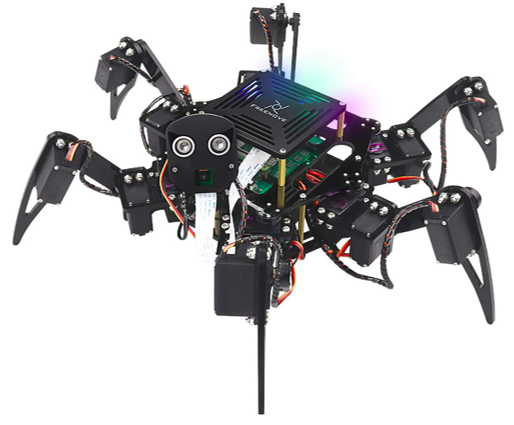
\includegraphics[scale=0.5]{02_introduction/figures/hexapod1.png}}
    \caption{Freenove Big Hexapod robot kit}
    %\label{fig:Hexapod}
\end{figure}